\chapter{Derivation of wave equations and numerical models of wave propagation}
\label{chap:1}

In this chapter, we will briefly recall how acoustic wave equations for a static medium and also for a moving medium can be derived from two fundamental equations in fluid dynamics i.e.
the equation of continuity and Euler's equation (Newton's second law). An acoustic wave will classically be introduced as a small adiabatic fluctuation of a fluid. The elastic wave
equation will then also be derived. The main ideas behind numerical modeling for wave propagation based on ray methods, Finite-Difference Time-Domain (FDTD) methods, Time-domain Finite Element Methods (FEM) and Spectral Element Methods (SEM) will also be briefly recalled. To conclude, a classical open-source numerical code for wave propagation called SPECFEM will be
briefly reviewed. In the next chapters we will use it extensively for our numerical simulations of ultrasonic wave propagation in parts of Sodium-cooled Fast Reactors (SFR).

\section{Summary of the main ideas behind the classical derivation of ultrasonic wave equations}

    \subsection{Acoustic wave propagation equation in a static medium}

        The basic equations for several types of acoustic wave propagation are generally derived from general aspects of continuum mechanics. This means that the
discontinuity caused from the molecular structure of matter may be ignored by considering it macroscopically. Those derivations start from two fundamental
equations in fluid dynamics (e.g., \cite{Landau1987Fluidmechanics}),
        i.e. the equation of continuity:
        \begin{align} \label{eq:1_1}
            \frac{\partial \tilde{\rho}}{\partial t} + \nabla \cdot (\tilde{\rho} \tilde{\bm{\nu}}) = 0,
        \end{align}
        and Euler's equation (Newton's second law):
        \begin{align} \label{eq:1_2}
            \frac{\partial \tilde{\bm{\nu}}}{\partial t} + (\tilde{\bm{\nu}} \cdot \nabla)\tilde{\bm{\nu}} = - \frac{1}{\tilde{\rho}}\nabla\tilde{p},
        \end{align}
        where $\tilde{\rho}$ stands for density, $t$ stands for time, $\tilde{\bm{\nu}}$ is the distribution of particle velocity, $\nabla$ represents a gradient
 $\nabla \cdot$ represents the divergence of a given physical quantity, and $\tilde{p}$ is pressure. Fields, quantities and components here and below
may depend on time $t$ and position $\bm{r}$ , e.g.
$\tilde{\bm{\nu}}(\bm{r},t) = \tilde{\bm{\nu}}(x,y,z,t)$ in three-dimensional Cartesian coordinates.

        A sound wave is introduced as an oscillatory motion with small amplitude in a compressible fluid, and this oscillation is considered approximately as an
adiabatic process. Thus the equation of state relating pressure and density and a condition for an isentropic process are added:
        \begin{align} \label{eq:1_3}
            \tilde{p}=\tilde{p}(\tilde{\rho},\tilde{S}),
        \end{align}
\vspace*{-7mm}
        \begin{align} \label{eq:1_4}
            \biggl( \frac{\partial}{\partial t} + \bm{\tilde{\nu}}\cdot\nabla \biggr)\tilde{S}=0,
        \end{align}
        where $\tilde{S}$ stands for entropy.
        Considering an isentropic or adiabatic process means that the diffusion of components in a fluid and the thermal conductivity are neglected
\parencite{Brekhovskikh1998AcousticsofLayered}.

        By multiplying both sides of equation \ref{eq:1_3} by the material derivative ($d/dt=\partial/\partial t + \bm{\nu_0} \cdot\nabla$) and expanding it with
total derivative, and substituting equation \ref{eq:1_4}, a relationship between density and pressure may be obtained:
        \begin{align} \label{eq:1_5}
            \biggl( \frac{\partial}{\partial t} + \bm{\tilde{\nu}}\cdot\nabla \biggr)\tilde{p}=\tilde{c}^2\biggl( \frac{\partial}{\partial t} +
\bm{\tilde{\nu}}\cdot\nabla \biggr)\tilde{\rho},
        \end{align}
        where $\tilde{c}^2 = \partial \tilde{p}(\tilde{\rho},\tilde{S}) / \partial \tilde{\rho}$ is the definition of the squared sound velocity, which includes the
fluctuation part caused by wave propagation, while the squared adiabatic sound speed is defined as $c^2_0 = \partial p(\rho_0,S_0) / \partial \rho_0$.

        In the above equations, source terms and also acceleration due to gravity are ignored for now. Thus each component in equations \ref{eq:1_1} to
\ref{eq:1_5} may be split in two parts as $\tilde{\rho}=\rho_0+\rho, \bm{\tilde{\nu}}=\bm{\nu_0}+\bm{\nu}$, $\tilde{p}=p_0+p$, $\tilde{S}=S_0+s$,
$\tilde{c}=c_0+c$. $\rho_0$, $\bm{\nu_0}$, $p_0$, $S_0$, $c_0$ are the values in the absence of the wave and $\rho$, $\bm{\nu}$, $p$, $s$, $c$ are fluctuations
caused by the sound wave.
        By substituting these split components into \ref{eq:1_1}, \ref{eq:1_2}, \ref{eq:1_3} and \ref{eq:1_5}, one gets governing equations for a fluid state
including the vibration of a sound wave:
        \begin{align} \label{eq:1_6}
            \frac{d\rho_0}{dt}+\rho_0\nabla\cdot\bm{\nu_0}+\frac{d\rho}{dt}+\nabla\cdot(\rho_0\bm{\nu})+\rho\nabla\cdot\bm{\nu_0}=0,
        \end{align}
\vspace*{-7mm}
        \begin{align} \label{eq:1_7}
            \frac{d\bm{\nu_0}}{dt}
            +\frac{1}{\rho_0}\nabla p_0
            +\frac{d\bm{\nu}}{dt}
            +(\bm{\nu}\cdot\nabla)\bm{\nu_0}\frac{\nabla p}{\rho_0}
            -\frac{\rho\nabla p_0}{\rho_0^2}=0,
        \end{align}
\vspace*{-7mm}
        \begin{align} \label{eq:1_8}
            \frac{dS_0}{dt}+\frac{ds}{dt}+(\bm{\nu}\cdot\nabla)S_0=0,
        \end{align}
\vspace*{-7mm}
        \begin{align} \label{eq:1_9}
            \frac{p_0}{dt}+\frac{dp}{dt}+(\bm{\nu}\cdot\nabla)p_0=
        c_0^2\biggl( \frac{d\rho_0}{dt}+\frac{d\rho}{dt}+(\bm{\nu}\cdot\nabla)\rho_0\biggr)+2c_0c\frac{d\rho_0}{dt}.
        \end{align}
        where $d/dt=\partial/\partial t+\bm{\nu_0}\cdot\nabla$ is a material derivative. All second-order terms (e.g. $(\bm{\nu}\cdot\nabla)\rho$ etc.) were
neglected by regarding them as small in this process called linearization, and the derived equations are thus the linearized wave equation.

        These four equations may again be divided into fluid mechanics equations for the ambient flow (by separating zero-order terms):
        \begin{align} \label{eq:1_10}
            \frac{d\rho_0}{d t}+\rho_0\nabla\cdot\bm{\nu_0}=0,
        \end{align}
\vspace*{-7mm}
        \begin{align} \label{eq:1_11}
            \frac{d\bm{\nu_0}}{d t}+\frac{1}{\rho_0}\nabla p_0=0,
        \end{align}
\vspace*{-7mm}
        \begin{align} \label{eq:1_12}
            \frac{d S_0}{d t}=0,
        \end{align}
\vspace*{-7mm}
        \begin{align} \label{eq:1_13}
            \frac{d p_0}{d t}=c_0^2\frac{d \rho_0}{d t}
        \end{align}
        and linear equations for the wave-induced perturbation:
        \begin{align} \label{eq:1_14}
            \frac{d \rho}{d t} + \nabla\cdot(\rho_0 \bm{\nu})+\rho\nabla\cdot\bm{\nu_0} = 0,
        \end{align}
\vspace*{-7mm}
        \begin{align} \label{eq:1_15}
            \frac{d \bm{\nu}}{d t} + (\bm{\nu}\cdot\nabla)\bm{\nu_0} + \frac{\nabla p}{\rho_0} - \frac{\rho\nabla p_0}{\rho_0^2}=0,
        \end{align}
\vspace*{-7mm}
        \begin{align} \label{eq:1_16}
            \frac{d s}{d t}+(\bm{\nu}\cdot\nabla)S_0=0,
        \end{align}
\vspace*{-7mm}
        \begin{align} \label{eq:1_17}
            \frac{d p}{d t}+(\bm{\nu}\cdot\nabla)p_0 = c_0^2 \biggl( \frac{d \rho}{d t} + \bm{\nu}\cdot\nabla\rho_0 \biggr) + 2c_0 c \frac{d \rho_0}{d t}
        \end{align}
        These four equations \ref{eq:1_14}, \ref{eq:1_15}, \ref{eq:1_16} and \ref{eq:1_17} are \textbf{the general linearized equations} for acoustic wave
propagation, excluding terms for a source and acceleration due to gravity, i.e. every component may change in time and space as well.

        If the sound speed is defined as $\tilde c^2 = c_0^2+c^2$ in equation \ref{eq:1_5}, equation \ref{eq:1_17} becomes
        \begin{align} \label{eq:1_18}
            \frac{d p}{d t}+(\bm{\nu}\cdot\nabla)p_0 = c_0^2 \frac{d \rho}{d t}+(c_0^2 + c^2)(\bm{\nu}\cdot\nabla)\rho_0
        \end{align}
        instead. The former formulation may be found for instance in \cite{Godin2011Anexactwave} and the latter in \cite{Brekhovskikh1998AcousticsofLayered}.

        In the case of a static medium, the term for the ambient flow $\bm{\nu}_0$ is equal to zero, which makes equations \ref{eq:1_14},\ref{eq:1_15},\ref{eq:1_17} or
\ref{eq:1_18} become:
        \begin{align} \label{eq:1_19}
            \frac{\partial \rho}{\partial t}+\nabla\cdot(\rho_0 \bm{\nu})=0,
        \end{align}
\vspace*{-7mm}
        \begin{align} \label{eq:1_20}
            \frac{\partial \bm{\nu}}{\partial t}+\frac{1}{\rho_0}\nabla p=0,
        \end{align}
\vspace*{-7mm}
        \begin{align} \label{eq:1_21}
            \frac{\partial p}{\partial t}=c_0^2\frac{\partial \rho}{\partial t},
        \end{align}
        where ambient pressure is assumed to verify $\nabla p_0=0$ (i.e. $d\bm{u_0}/dt$ from \ref{eq:1_11}). Also, from $\bm{\nu_0}=0$, \ref{eq:1_10} and \ref{eq:1_13},
$d\rho_0/d t$, $d p_0/dt=0$ are enforced automatically. In this assumption the type of ambient flows is limited, but it can still be time-dependent i.e. unsteady,
and also spatially heterogeneous.

        By substituting \ref{eq:1_19} into \ref{eq:1_21} in order to cancel $\partial \rho/\partial t$, then differentiating it partially in time and
substituting \ref{eq:1_20} to eliminate $\partial \bm{\nu}/\partial t$, \textbf{the wave equation for pressure} is derived as:
        \begin{align} \label{eq:1_22}
            \frac{\partial}{\partial t}\biggl(\frac{1}{\rho_0 c_0^2}\frac{\partial p}{\partial t} \biggr) - \nabla\cdot\biggl(\frac{1}{\rho_0}\nabla p
\biggr)=0.
        \end{align}
        In this equation, $\bm{\nu_0}=0$ and $\nabla p_0=0$ are assumed. This formulation is thus usable for wave propagation in a heterogeneous,
non-steady-state medium at rest \parencite{Brekhovskikh1998AcousticsofLayered}.

        By adding some assumptions to \ref{eq:1_22}, i.e. by making the assumptions $\bm{\nu_0}=0$, $\nabla p_0=0$, $\nabla \rho_0=0$ and $\partial
\rho_0/\partial t = \partial c_0 / \partial t = 0$, one obtains the simpler form:
        \begin{align} \label{eq:1_23}
            \nabla^2 p-\frac{1}{c_0^2}\frac{\partial^2 p}{\partial t^2}=0.
        \end{align}
        This equation is valid for a homogeneous, steady-state medium.
        In the same way, the wave equation for density perturbation may be derived as well.

        One can also derive \textbf{the wave equation for particle velocity} by taking the divergence of equation \ref{eq:1_19} and the time derivative of
\ref{eq:1_20}, and then combining them using \ref{eq:1_21} to get the wave equation for particle velocity as:
        \begin{align} \label{eq:1_24}
            \frac{1}{\rho_0}\nabla(c_0^2\nabla\cdot(\rho_0\bm{\nu}))-\frac{\partial^2 \bm{\nu}}{\partial t^2} = 0.
        \end{align}
        By using the relation between particle velocity $\bm{\nu}$ and particle displacement $\bm{u}$, i.e. $\bm{\nu}=\partial \bm{u}/\partial t$, the
wave equation for particle displacement is derived in the same way:
        \begin{align} \label{eq:1_25}
            \frac{1}{\rho_0}\nabla(c_0^2\nabla\cdot(\rho_0\bm{u}))-\frac{\partial^2 \bm{u}}{\partial t^2} = 0.
        \end{align}
        This transform is possible because one has already assumed time-independent density and sound velocity here.

        By assuming that density and sound speed is spatially constant, equation \ref{eq:1_25} may be rewritten with the same form as with pressure equation
\ref{eq:1_23}:
        \begin{align} \label{eq:1_26}
            \nabla^2 \bm{u}-\frac{1}{c_0^2}\frac{\partial^2 \bm{u}}{\partial t^2}=0.
        \end{align}

        Velocity and displacement forms are more rarely used because they are vectorial rather than scalar and also because they involve spatial derivatives of density and
sound velocity.

        Next, the \textbf{wave equation for a displacement potential} can also derived. The displacement scalar potential $\chi$ is defined by:
        \begin{align} \label{eq:1_27}
            \bm{u}=\nabla\chi
        \end{align}
        Using the displacement potential, one may derive a simple equation without having to assume that sound velocity is spatially constant,
but having to make such an assumption for density. After inserting \ref{eq:1_27} into \ref{eq:1_25} the equation below is obtained:
        \begin{align} \label{eq:1_28}
            \frac{1}{\rho_0}\nabla\biggl( \rho_0 c_0^2 \nabla^2\chi-\frac{\partial^2 \chi}{\partial t^2} \biggr)=0.
        \end{align}
        To satisfy this equation,
        \begin{align} \label{eq:1_29}
            \nabla^2\chi-\frac{1}{c_0^2}\frac{\partial^2 \chi}{\partial t^2}=0
        \end{align}
        is sufficient.

        Another way to define a scalar potential is to resort to a potential of "density times displacement":
        \begin{align} \label{eq:1_30}
            \rho_0\bm{u}=\nabla\chi.
        \end{align}
        By substituting \ref{eq:1_30} to \ref{eq:1_20}, this definition of potential may be written as:
        \begin{align} \label{eq:1_30b}
            p=-\ddot{\chi}.
        \end{align}
        By combining \ref{eq:1_30b} and \ref{eq:1_23}, we get:
        \begin{align} \label{eq:1_31}
            \ddot\chi - c_0^2\nabla\cdot\nabla\chi = 0,
        \end{align}
        or, using the acoustic bulk modulus $\lambda=\rho_0c_0^2$,
        \begin{align} \label{eq:1_32}
            \frac{1}{\lambda}\ddot\chi=\frac{1}{\rho}\nabla\cdot\nabla\chi.
        \end{align}
        This formulation is used in SPECFEM \parencite{Cristini2012Someillustrativeexamples} because of its advantages in implementation, which automatically
suppresses numerical artefacts that are known for appearing in the displacement formulation \parencite{Hamdi1978Adisplacementmethod}.


    \subsection{Acoustic wave propagation equation in a moving medium}

        Equations \ref{eq:1_14}, \ref{eq:1_15}, \ref{eq:1_16}, \ref{eq:1_17} or \ref{eq:1_18} already include the description of wave propagation in a
heterogeneous moving medium. These equations, however, may be transformed into simpler forms by applying restrictions for physically-realizable fluid flows.
        The derivation of the wave equation in moving heterogeneous media can be found for instance in \cite{VladimirE.Ostashev2015AcousticsMovingInhomogeneous}.
        In \cite{Godin2011Anexactwave}, a closed-form equation for acoustic pressure is derived.
First, some assumptions regarding the type of ambient flow are made:
        \begin{align} \label{eq:1_33}
            \frac{d \bm{\nu_0}}{d t} = 0,
        \end{align}
\vspace*{-7mm}
        \begin{align} \label{eq:1_34}
            \frac{d}{d t}(\nabla\nu_j)=0, j= 1,2,3,
        \end{align}
\vspace*{-7mm}
        \begin{align} \label{eq:1_35}
            \nabla\cdot\bm{\nu_0}=0.
        \end{align}
        From relations between these three conditions and equation \ref{eq:1_10}, \ref{eq:1_11}, \ref{eq:1_13}, $d\rho_0/d t=0$, $d p_0/d t=0$,$dc_0/d t=0$ and
$\nabla p_0=0$  are implied. The general linearized wave equations \ref{eq:1_14},\ref{eq:1_15} and \ref{eq:1_17} may then be simplified as:
        \begin{align} \label{eq:1_36}
            \frac{d \rho}{d t}+\rho_0\nabla\cdot\bm{\nu}+(\bm{\nu}\cdot\nabla)\rho_0= 0,
        \end{align}
\vspace*{-7mm}
        \begin{align} \label{eq:1_37}
            \frac{d\bm{\nu}}{d t}+(\bm{\nu}\cdot\nabla)\bm{\nu_0}+\frac{\nabla p}{\rho_0}=0,
        \end{align}
\vspace*{-7mm}
        \begin{align} \label{eq:1_38}
            \frac{d p}{d t}=c_0^2\biggl( \frac{d \rho}{d t}+(\bm{\nu}\cdot\nabla)\rho_0 \biggr).
        \end{align}
        From \ref{eq:1_36} and \ref{eq:1_38}, $d \rho/d t$ may be eliminated and one obtains
        \begin{align} \label{eq:1_39}
            \frac{1}{\rho_0 c_0^2}\frac{d p}{d t}+\nabla\cdot\bm{\nu}=0.
        \end{align}
        By applying the divergence operator to equation \ref{eq:1_37} and $d/dt$ to \ref{eq:1_39}, one gets
        \begin{align} \label{eq:1_40}
            \frac{d}{d t}\biggl( \frac{1}{\rho_0 c_0^2}\frac{d p}{d t} \biggr) - \nabla\cdot\frac{\nabla p}{\rho_0} =2\frac{\partial \nu_{0k}}{\partial
x_i}\frac{\partial \nu_i}{\partial x_k}
        \end{align}
        Here $j,k$ are indices following the Einstein notation convention of implicit sum over repeated indices.
These indices come from the divergence of the second term in the left-hand side of \ref{eq:1_37}, i.e.
$\nabla\cdot((\bm{\nu\cdot\nabla})\bm{\nu_0})$ and also from $\nabla\cdot(\frac{d\bm{\nu}}{d t})-\frac{d}{d t}(\nabla\cdot\bm{\nu})$. Also, considering the
difference between $\nabla(\frac{d\bm{\nu}}{d t})$ and $\frac{d}{d t}(\nabla\bm{\nu})$, equation \ref{eq:1_35} and \ref{eq:1_37} become
        \begin{align} \label{eq:1_41}
            \frac{d}{d t}\frac{\partial \nu_i}{\partial x_k}=\frac{\partial}{\partial x_k}\frac{d \nu_i}{d t}-\frac{\partial \nu_i}{\partial x_j}\frac{\partial
\nu_{0j}}{\partial x_k}
            =-\frac{\partial}{\partial x_k}\biggl(\frac{1}{\rho_0}\frac{\partial p}{\partial x_i}\biggr)+\nu_j\frac{\partial^2 \nu_{0j}}{\partial x_j \partial
x_k}+\frac{\nu_j}{\partial x_k}\frac{\partial \nu_{0i}}{\partial{x_j}}-\frac{\partial \nu_i}{\partial x_j}\frac{\partial \nu_{0j}}{\partial x_k},
        \end{align}
        and using \ref{eq:1_34} we get
        \begin{align} \label{eq:1_42}
            \frac{d}{d t}\biggl( \frac{\partial \nu_{0k}}{\partial x_i}\frac{\partial \nu_i}{\partial x_k} \biggr) = -\frac{\partial \nu_{0k}}{\partial
x_i}\frac{\partial}{\partial x_k}\biggl(\frac{1}{\rho}\frac{\partial p}{\partial x_i}\biggr).
        \end{align}
        After applying $d/dt$ to equation \ref{eq:1_40} and then combining it with \ref{eq:1_42}, \textbf{the acoustic wave equation for pressure in a heterogeneous moving medium} is derived,
        \begin{align} \label{eq:1_43}
            \frac{d}{d t}\biggl[ \frac{d}{d t}\biggl( \frac{1}{\rho_0 c_0^2}\frac{d p}{d t}- \nabla\cdot \frac{\nabla p}{\rho_0}\biggr)\biggr]+2\frac{\partial
\bm{\nu_0}}{\partial x_i}\cdot\nabla\biggl(\frac{1}{\rho}\frac{\partial p}{\partial x_i}\biggr)=0.
        \end{align}
        Let us note that this equation includes a third-order time derivative, which may be difficult to handle in classical numerical time-marching schemes.


    \subsection{Elastic wave propagation equation}

        From Newton's second law, the total body force and surface force and the kinematic state of a volume $V$ and its surface $S$ satisfy the condition
        \begin{align} \label{eq:1_44}
            \frac{d}{d t}\int_V\rho\bm{\nu}dV=\int_S\bm{n}\cdot\bm{T}dS + \int_V\rho\bm{f}dV,
        \end{align}
        where $\rho$ is density, $\bm{\nu}$ is particle velocity, $\bm{T}$ is the stress tensor, $\bm{f}$ is a body force and $\bm{n}$ is an outward unit normal vector.
Here $d/dt$ is again a material derivative. By applying Gauss' theorem
(i.e. $\frac{d}{dt}\int_V\rho\bm{\nu}dV=\int_V\rho\frac{d\bm{\nu}}{d t}dV$) this equation becomes,
        \begin{align} \label{eq:1_45}
            \int_V\biggl[\nabla\cdot\bm{T}+\rho\bm{f}-\rho\frac{d\bm{\nu}}{d t}\biggr]dV=0.
        \end{align}
        This integral is valid everywhere in an arbitrary volume:
        \begin{align} \label{eq:1_46}
            \nabla\cdot\bm{T}+\rho\bm{f}-\rho\frac{d\bm{\nu}}{d t}=0.
        \end{align}
        This equation is Cauchy's \textbf{equation of motion} i.e. Euler's equation.

        Applying the small deformation approximation in the material derivation of particle velocity leads to
        \begin{align} \label{eq:1_47}
            \frac{d \bm{u}}{d t}= \frac{\partial \bm{u}}{\partial t}+ (\bm{\nu}\cdot\nabla)\bm{u}\cong\frac{\partial \bm{u}}{\partial t}\: and\:
\frac{d\bm{\nu}}{d t}=\frac{\partial \bm{\nu}}{\partial t}+(\bm{\nu}\cdot\nabla)\bm{\nu}\cong\frac{\partial^2\bm{u}}{\partial t^2}.
        \end{align}
        Then \ref{eq:1_46} may be expressed as
        \begin{align} \label{eq:1_48}
            \nabla\cdot\bm{T}+\rho\bm{f}=\rho\frac{\partial^2 \bm{u}}{\partial t^2}=\rho\ddot{\bm{u}}.
        \end{align}
The strain tensor is $\epsilon_{ij}=\frac{1}{2}(u_{i,j}+u_{j,i})$, with the notation $u_{i,j}=\partial_i / \partial x_j$.
        In the elastic solid, the relation between stress and strain, i.e. Hooke's law, can be expressed as
        \begin{align} \label{eq:1_49}
            \tau_{ij}=C_{ijkl}\epsilon_{kl},
        \end{align}
        where $\tau_{ij}$ are the components of the stress tensor, $\epsilon_{kl}$ are the components of the strain tensor,
and $C_{ijkl}$ are the components of the fourth-order elastic stiffness tensor.

        For isotropic materials, Hooke's law has the simpler expression
        \begin{align} \label{eq:1_50}
            \tau_{ij}=\lambda\delta_{ij} \epsilon_{kk}+ 2\mu\epsilon_{ij}=\lambda\delta_{ij} u_{k,k}+\mu(u_{i,j}+u_{j,i}),
        \end{align}
where $\lambda$ and $\mu$ are the two Lam\'e parameters, and $\delta_{ij}$ is the Kronecker delta symbol, which is equal to 1 when $i = j$ and to zero otherwise.

\section{A few classical numerical methods to simulate wave propagation}

    There exists several classical ways to numerically model wave propagation in complex media. These methods are divided broadly into two parts: ray-based methods,
and full wave methods. Each has its own pros and cons, and thus an appropriate modeling method should be chosen depending on the purpose of a given calculation,
and also on the numerical cost that one is willing to pay.
    Usually, ray-based methods are used in situations in which  the computation speed and cost of computational resources are important.
    Full wave methods, including FDTD, time-domain or frequency-domain FEM, and SEM, are used when problems require high accuracy, and/or when cost is a less critical issue, or can be afforded.

    \subsection{Ray-based methods}

        Ray-based models have been used for many years in optics, electromagnetics, seismology and acoustics. Ray theory was first developed in optics,
which initially considered only the deflection from Snell's law, but nowadays ray methods are increasingly varied and also sophisticated.
        In the scientific community, nowadays the use of ray methods is not the usual choice because its high-frequency (in fact, infinite frequency) approximation leads to a degradation of the accuracy
\parencite{Jensen2011ComputationalOceanAcoustics}. However, these methods are still sometimes chosen because of their great advantages in terms of calculation speed
and low computational resources.
In recent application studies for sodium-cooled fast reactors, as presented in Chapter \ref{chap:1}, \textcite{Massacret2014Modellingofultrasonic} used a ray method for
the analysis of inhomogeneity effects on sound propagation taking into account temperature gradients and flow velocities.
\textcite{Lue2012Stochasticsimulationof} developed a faster and more efficient ray-tracing method for inhomogeneous media.
In this method, an acoustic field is initially calculated for a homogeneous medium, and then the effect of the heterogeneity of the medium is calculated
for only specific spatial positions instead of calculating it for the fluctuating medium in the whole simulated region.
\textcite{Lue2016Numericalcomparisonof} made a detailed comparison study between multiple ray-tracing methods in terms of accuracy of reflection/scattering phenomena
for a wedge model, i.e. a reflective object that has an edge with a shallow angle.
The commercial software "CIVA" for sound propagation analysis also uses such a technique, in a better and more modern approach based on so-called "fat rays" or "pencils".
It therefore performs ray tracing in inhomogeneous and anisotropic elastic media based on such a pencil technique \parencite{Gengembre2000Pencilmethodin}.
The studies that apply ray-based method are presented in Chapter \ref{chap:1}.

    \subsection{Finite Differences in the Time Domain (FDTD) methods}
    \label{ssec:fdtd}

        Finite Differences in the Time Domain (FDTD) methods were initially introduced by \textcite{Yee1966Numericalsolutionof} as a numerical simulation method for electromagnetic fields,
with work by \cite{Cho68} on this technique for the Navier-Stokes equations, also at the end of the 1960s.
This method was then applied for acoustics, for example ocean acoustics and seismology \citep{Mad76,ViMa82,Vir84,Vir86,SaGoSh00,MiKo10}.
        In a finite-difference scheme, the spatial domain is discretized as grid points, which are usually evenly-spaced, and all physical properties are
defined only at these fixed grid points (or also in the middle between these grid points, in the case of so-called spatially-staggered schemes).
This restriction on the placement of physical values, as well as the use of symmetric differentiation operators,
which would require fictitious grid points located beyond the boundary, causes difficulties for accurate expressions of material boundaries and of boundary conditions,
especially if the shape has complex geometry. There are several studies on FDTD methods for media that include curved boundaries (e.g.
\textcite{Jurgens1992Finitedifferencetime,MoByKrCaBo97,KrMo03,Tarrass11}) which use e.g. an interpolation method based on the distance between a discretized point and a (potentially curved) boundary,
but they are only partially satisfactory in terms of accuracy and also make FDTD techniques more complex, thus partially losing one of their main advantages, which is their simplicity.

        The general derivation of finite difference (FD) schemes starts from expanding a sufficiently-smooth function spatially by performing a Taylor expansion:
        \begin{align} \label{eq:fdtd_1}
            f(x+h)=f(x)+h \frac{\partial f(x)}{\partial x}+\frac{1}{2}h^2 \frac{\partial^2 f(x)}{\partial^2 x}+\cdots,
        \end{align}
\vspace*{-4.5mm}
        \begin{align} \label{eq:fdtd_2}
            f(x-h)=f(x)-h \frac{\partial f(x)}{\partial x}+\frac{1}{2}h^2 \frac{\partial^2 f(x)}{\partial^2 x}-\cdots,
        \end{align}
        where, in a 1D example, $x$ is the coordinate of a point at which the partial derivative of $f(x)$ is approximated, and $h$ is the spatial grid-cell size.
By subtracting \ref{eq:fdtd_2} from \ref{eq:fdtd_1} FD schemes can compute partial derivatives.
Depending on the order (in terms of powers of $h$) of the terms which cancel out and of the terms that remain as residuals, variable types of FD schemes have been
proposed. Nowadays, in many cases a staggered grid is used to improve the order of convergence, i.e. $h=\Delta x/2$ where $\Delta x$ is the grid spacing, and some unknowns
are located half way between grid points.
        The first-order derivative is approximated as:
        \begin{align} \label{eq:fdtd_3}
            \frac{\partial f(x)}{\partial x}\approx \frac{d_xf(x)}{2h}.
        \end{align}
        $d_xf(x)$ is the Finite Difference (FD) operator.

        Below is an example of the simplest case of a second-order FD operator, of second-order accuracy:
        \begin{align} \label{eq:fdtd_4}
             d_x f(x)=f(x+h)-f(x-h).
        \end{align}
        The fourth-order accurate FD operator is:
        \begin{align} \label{eq:fdtd_5}
             d_x f(x)=c_1 [f(x+h)-f(x-h)] + c_2 [f(x+3h)-f(x-3h)],
        \end{align}
        with $c_1=9/8, c_2=-1/24$ \parencite{Levander1988Fourthorderfinite}.
        In the wave equation for a static acoustic medium
        \begin{align} \label{eq:fdtd_6}
            \frac{1}{\rho_0 c_0^2} \frac{\partial^2 p}{\partial t^2}=\nabla \cdot (\frac{1}{\rho_0}\nabla p),
        \end{align}
        where $\rho_0$ and $c_0$ are ambient values of the propagation medium and $p$ is the fluctuation of pressure,
        the FD operator can be applied twice to the first-order spatial derivative in one time step to calculate the values of the
right-hand side of \ref{eq:fdtd_6}. One can then for instance use a Newmark scheme for temporal discretization \citep{Hug87} to calculate the pressure values at the next time step.
        These are classical FDTD schemes developed until the end of the 1980s. Based on these classical methods, the development of FDTD techniques has continued
in the community over the years in order to improve the accuracy and stability of the methods, in particular by going to higher-order operators in
terms of Taylor expansion (e.g. in \ref{eq:fdtd_1} and \ref{eq:fdtd_2}).

        In our study, we applied two classical FD schemes, i.e. classical second-order and fourth-order, and two more modern methods called Non-standard FDTD
\parencite{JafarGandomi2009NonstandardFDTD} and Fourth-order optimized FD \parencite{Bilbao2013Constructionandoptimization}. In these latter modern FD schemes,
the nodes (or grid points) used to calculate a FD operator for one direction are not limited only to the line of points going in that direction, but rather spreading in two
dimensions or three dimensions, depending on the spatial dimension of the problem.
The distribution of these nodes is called a "stencil", and each FD scheme has its shape of stencil. Below we recall the main ideas in these two modern schemes.

\noindent
        \underline{\textbf{Non-standard FDTD}}

            The main idea of the Non-standard FDTD scheme is to optimize the scheme for a sine wave with fixed frequency by introducing parameters to be optimized.
In Non-standard FDTD, the FD operator is defined as:
            \begin{align} \label{eq:fdtd_7}
                \frac{\partial f(x)}{\partial x} \approx \frac{d_x f(x)}{S(\Delta x)},
            \end{align}
            where $S(\Delta x)$ is the so-called correction function. Second- and fourth-order correction functions are derived respectively by replacing $f(x)$
with a plane wave solution $e^{ikx}$ ($k$ being the wave number),
            \begin{align} \label{eq:fdtd_8}
                S_{2nd}(\Delta x) = \frac{2}{k} sin(\frac{k \Delta x}{2}),
            \end{align}
\vspace*{-7mm}
            \begin{align} \label{eq:fdtd_9}
                S_{4th}(\Delta x) = \frac{2}{k} sin(c_1 \frac{k \Delta x}{2} + c_2 \frac{3k \Delta x}{2}).
            \end{align}
            A correction function is also defined for the time step $\Delta t$ in the same manner:
            \begin{align} \label{eq:fdtd_10}
                S_{t,2nd}(\Delta t)=\frac{2}{\omega}sin\left( \frac{\omega\Delta t}{2} \right),
            \end{align}
\vspace*{-7mm}
            \begin{align} \label{eq:fdtd_11}
                S_{t,4th}(\Delta t)=\frac{2}{\omega}sin\left( c_1\frac{\omega\Delta t}{2} + c_2\frac{3\omega \Delta t}{2} \right).
            \end{align}

            In fourth-order Non-standard FDTD, two FD operators are defined for each spatial dimension. In the 2D case,
            \begin{align} \label{eq:fdtd_12}
                d^{(1)}_{x,\Delta x}f(x,z)=f\left(x+\frac{\Delta x}{2},z\right)-f\left(x-\frac{\Delta x}{2},z\right),
            \end{align}
\vspace*{-7mm}
            \begin{align} \label{eq:fdtd_13}
                d^{(2)}_{x,\Delta x}f(x,z)=\frac{1}{2}\left[f\left(x+\frac{\Delta x}{2},z+\Delta z\right)-f\left(x-\frac{\Delta x}{2},z+\Delta z\right) \right.
\nonumber \\
                \left. +f\left(x+\frac{\Delta x}{2},z-\Delta z\right)-f\left(x-\frac{\Delta x}{2},z-\Delta z\right)\right]
            \end{align}
            \cite{JafarGandomi2009NonstandardFDTD} introduce a broader stencil that uses the additional two FD operators below:
            \begin{align} \label{eq:fdtd_14}
                d^{(1)}_{x,3\Delta x}f(x,z)=f\left(x+\frac{3\Delta x}{2},z\right)-f\left(x-\frac{3\Delta x}{2},z\right),
            \end{align}
\vspace*{-7mm}
            \begin{align} \label{eq:fdtd_15}
                d^{(2)}_{x,3\Delta x}f(x,z)=\frac{1}{2}\left[f\left(x+\frac{3\Delta x}{2},z+3\Delta z\right)-f\left(x-\frac{3\Delta x}{2},z+3\Delta z\right)
\right. \nonumber \\
                \left. +f\left(x+\frac{3\Delta x}{2},z-3\Delta z\right)-f\left(x-\frac{3\Delta x}{2},z-3\Delta z\right)\right]
            \end{align}
            FD operators for the $z$ direction are straightforwardly obtained by replacing $x$ with $z$.
            Finally, the parameters to be optimized are introduced in the definition of the fourth-order FD Laplacian:
            \begin{align} \label{eq:fdtd_16}
                D^{(0)}_{4th}=\frac{d^{(1)}_x d^{(0)}_x}{[S_{4th} \Delta x]^2}+\frac{d^{(1)}_z d^{(0)}_z}{[S_{4th} \Delta z]^2},
            \end{align}
            where
            \begin{align} \label{eq:fdtd_17}
                d^{(i)}_x = c_1 d^{(i)}_{x, \Delta x} + c_2 d^{(i)}_{x,3\Delta x}\ (i=0,1),
            \end{align}
\vspace*{-7mm}
            \begin{align} \label{eq:fdtd_18}
                d^{(0)}_{x,\Delta x} = q_1 d^{(1)}_{x,\Delta x} + (1-q_1) d^{(2)}_{x,\Delta x},
            \end{align}
            and for broader stencil
            \begin{align} \label{eq:fdtd_19}
                d^{(0)}_{x,3\Delta x} = q_2 d^{(1)}_{x,3\Delta x} + (1-q_2) d^{(2)}_{x,3\Delta x},
            \end{align}
            where $q_1$ and $q_2$ are the parameters to be optimized.
Again, these FD operators for the $z$ direction can be obtained by replacing $x$ with $z$ in each formulation.
            $q_1$, $q_2$ are obtained by minimizing the equation
            \begin{align} \label{eq:fdtd_20}
                dk^2=\int^{\pi/2}_0 \left| \frac{D^{(0)}_{4th}f(x,z)}{f(x,z)} + |\bm{k_0}|^2 \right| d\theta,
            \end{align}
            where the wave vector $\bm{k_0}=(k_0 sin\theta, k_0 cos\theta)$ and $f(x,y) = e^{i\bm{k_0}\cdot \bm{r}}\  (\bm{r}=(x,z))$ is substituted when this
optimization problem is solved.
            This equation minimizes the numerical dispersion error, i.e. the difference between the numerical and analytical phase velocities (\parencite{Ohtani2005Newoptimizationparameters}).
            Applying this operator to the wave equation (right-hand side of \ref{eq:fdtd_6}) leads to the approximated version
            \begin{align} \label{eq:fdtd_21}
                \frac{1}{\rho_0 c_0^2} \frac{d^2_t p}{S_t^2(\Delta t)} = \left[\frac{d^{(1)}_x}{S_{4th}(\Delta x)}_x,\frac{d^{(1)}_z}{S_{4th}(\Delta
z)}\right]\cdot \frac{1}{\rho_0}\left[\frac{d^{(0)}_x}{S_{4th}(\Delta z)}, \frac{d^{(0)}_z}{S_{4th}(\Delta z)}\right]^Tp,
            \end{align}
            where $[]^T$ denotes the transpose of a vector.
            Values calculated by the first application of FD operators, i.e. the right-hand side of the center dot in \ref{eq:fdtd_21},
are stored at all the middle nodes of the staggered grid, and then, when the FD operators are applied a second time, i.e. for the left-hand side of the center dot,
they allow for the calculation of the second-order time-derivative at all the grid points.

\noindent
        \underline{\textbf{Fourth-order optimized FDTD}}

        In this method, the FD approximation is applied directly to the Laplacian operator, i.e. to second-order spatial derivatives,
rather than applying FD operators for first-order spatial derivatives twice. This leads to a significant reduction of the calculation cost, of about a factor of two.
However, this means that the medium is assumed to be locally homogeneous, or with very smooth and small local variations, to make it possible to neglect the gradient of the
physical parameters and convert the operator to a Laplacian.
In this case, the following wave equation is used:
            \begin{align} \label{eq:fdtd_22}
                \frac{1}{\rho_0 c_0^2}\frac{\partial^2 p}{\partial t^2}= \frac{1}{\rho_0}\Delta p
            \end{align}
            where $\Delta$ is the Laplacian. The term $1/\rho_0$ is moved out of the gradient because the air is considered homogeneous.
This means that this equation and this scheme models the
propagation medium without any change of temperature nor wave speed, or extremely smooth variations.
This can be valid in the case of aeroacoustics, however using such an approximation for a sodium reactor is more problematic.
            From \ref{eq:fdtd_1} and \ref{eq:fdtd_2}, the second-order partial derivative of a function in 1D becomes
            \begin{align} \label{eq:fdtd_23}
                \frac{\partial^2 f(x)}{\partial x^2} = \frac{f(x-h)-2f(x)+f(x+h)}{h^2} \mathrm{ \ + \ residuals},
            \end{align}
            where $h$ is the size of a grid cell. When the FD operator is applied to the Laplacian, the half grid step is no longer necessary because the approximation
of the second-order derivative does not involve staggered grid points.

            \begin{figure}[htbp]
                     \centerline{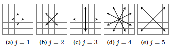
\includegraphics[keepaspectratio,width=90mm]{fdtd1.pdf}}
                \slantedcaption{Visual representation of $\bm{\nu_i}$ in each partial stencil $\Omega_i$ \parencite{Bilbao2013Constructionandoptimization}.}
                \label{fig:b1}
             \end{figure}

            The FD operator, which cancels the residuals in \ref{eq:fdtd_23}, is then applied by introducing the two-dimensional 25-point stencil
and the coefficients to be optimized:
            \begin{align} \label{eq:fdtd_24}
                D_{\Delta,\bm{\alpha},\bm{\gamma}}f(\bm{r})=\sum^5_{j=1}\alpha_j \frac{\kappa_j}{h^2}\sum^{|\Omega_j|}_{i=1}
\left(f(\bm{r}+\bm{v_i}h)-2f(\bm{r})+f(\bm{r}-\bm{v_i}h)\right),
            \end{align}
            where the position vector is $\bm{(x,z)}$, and the parameters $\bm{\alpha}\in\mathbb{R}^5$ are optimized based on the condition
            \begin{align} \label{eq:fdtd_25}
                \sum^5_{j=1}\alpha_j=1
            \end{align}
            corresponding to partial stencils divided into 5 parts from the whole 25-point stencil $\Omega\subset\mathbb{R}^2,\ \Omega=\sum^5_{i=1}\Omega_i$.
            Vector elements (for instance in \ref{eq:fdtd_24}) included in each partial stencil may be expressed with 2D Cartesian basis vectors $\bm{e_x},\bm{e_y}$,
            \begin{align} \label{eq:fdtd_26}
                \Omega_1 &=& \left[ \bm{e_x}, \bm{e_z} \right],\nonumber \\
                \Omega_2 &=& \left[ \bm{e_x}\pm\bm{e_z} \right],\nonumber \\
                \Omega_3 &=& 2\Omega_1, \nonumber \\
                \Omega_4 &=& \left[ 2\bm{e_x}\pm\bm{e_z}, \bm{e_x}\pm2\bm{e_z} \right], \nonumber \\
                \Omega_5 &=& 2\Omega_2
            \end{align}
            and
            \begin{align} \label{eq:fdtd_27}
                \kappa_j = \frac{2}{|\Omega_j| ||\bm{v}||^2},
            \end{align}
            where $|\Omega_j|$ is the index of the vector and $||\bm{v}||^2$ is the second-order norm (Euclidean norm) of any $\bm{v}_i \in \Omega_j$.

            \ref{fig:b1} shows the visual representation of the partial stencils. One finally uses $\bm{\Upsilon}=[\Omega_1,\Omega_2,\Omega_3,\Omega_4,\Omega_5]$.
            The optimized parameters $\bm{\alpha}$ are obtained by minimizing the relative phase velocity for the wave vector.
            More details may be found in \cite{Walstijn2008Onthenumerical} and \cite{Bilbao2013Constructionandoptimization}.
            \ref{fig:b2} shows the drawing of stencils of each of the FDTD schemes that we consider. Only the stencils for the $x$ direction are shown, except for the optimized FDTD scheme, which is 2D by design
and thus cannot be split into independent 1D components.
            \begin{figure}[htbp]
                    \centerline{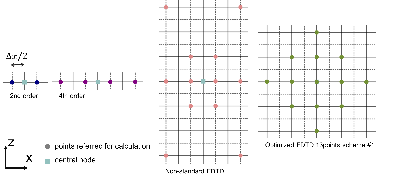
\includegraphics[keepaspectratio,width=150mm]{fdtd2.pdf}}
                \slantedcaption{Stencils for each of the FD schemes that we consider. The function value at the central node is calculated from the values at points represented by the circular
symbols. Only the stencils for the $x$ direction are shown, except for the optimized FDTD scheme, which is 2D by design
and thus cannot be split into independent 1D components.}
                \label{fig:b2}
             \end{figure}

\noindent
        \underline{\textbf{Compact schemes}}

             The main idea of compact FD schemes is to consider the calculation of FD-approximated spatial derivatives in 1D obtained by solving a 2D linear system, and then
obtain the spatial derivatives of not only one point but also its adjacent point at the same time. Here is the general derivation taken from \cite{Hixon2000Prefactoredsmallstencil} for the 1D case:
            \begin{align} \label{eq:fdtd_28}
                [B]\left[D\right]=\frac{1}{\Delta x}[C][f],
            \end{align}
            where $D$ is a 1D matrix that includes spatial derivatives of function $f$, and $B$ is a 2D matrix of coefficients. $C$ is also a 2D matrix of
coefficients. The expansion of \ref{eq:fdtd_28} at point $i$ at eighth order is then
            \begin{align} \label{eq:fdtd_29}
                \gamma(D_{i+2}+D_{i-2})+\beta(D_{i+1}+D_{i-1})+(1-\gamma-\beta)D_i\\
                = \frac{1}{\Delta x}\left[ \varphi(f_{i+2}+f_{i-2})+\eta(f_{i+1}+f_{i-1}) \right].
            \end{align}
            When gamma and beta are both zero, this becomes the equation for an explicit scheme. The spatial derivatives are then obtained:
            \begin{align} \label{eq:fdtd_30}
                [D]=[B]^{-1}\frac{1}{\Delta x}[C][f].
            \end{align}
            In \cite{Hixon2000Prefactoredsmallstencil}, $D$ is split in two parts in order to change the $B$ matrix from tridiagonal to bidiagonal for
fourth and sixth-order schemes. This scheme was initially developed for aeroacoustics but has also been successfully applied to linear wave propagation phenomena
\parencite{Rona2017Optimisedprefactoredcompact}.

    \subsection{Time domain Finite-Element Method and Spectral-Element Method}
    \label{ssec:sem}

        In order to distinguish from the case of static problems (e.g. a small deformation problem of solid mechanics), finite element methods when applied to dynamic problems
are sometimes referred to as Finite-Element Time-Domain methods (FETD or TDFE).
        The main difference between FETDs and the Spectral-Element Method (SEM) will be recalled below; it is mostly the fact that Gauss-Lobatto-Legendre points will be used,
while Gauss points are used in classical FETDs.
In other words, the SEM uses higher-order basis functions and a modified formulation that leads to a perfectly diagonal mass matrix, thus trying to combine the geometrical
flexibility of classical finite-element methods with the high accuracy of pseudospectral methods.
        Spectral methods are a class of discretization for differential equations, whose theory was for instance detailed by
\textcite{Gottlieb1977Numericalanalysisof}, and then in the 1980s spectral methods began to be applied for problems involving complex domains or media.
The SEM itself was introduced for computational fluid dynamics by \textcite{Patera1984Aspectralelement}, and later became very successful and widely used to
model the propagation of seismic wave in seismology \citep{KoTr99,Fic10,Peter2011Forwardandadjoint}
because the SEM can handle complex shapes of model boundaries in the simulated domain and also may
accurately compute surface waves. In addition, the SEM can easily model the anisotropy of a propagation medium \parencite{Komatitsch2000Simulationofanisotropic} as well as
fluid-solid boundaries \parencite{Komatitsch2000Wavepropagationnear}.

\clearpage
\noindent
        \underline{\textbf{Finite-element discretization}}

            In a finite-element discretization, a domain $\Omega$ is divided into a set of non-overlapping elements $\Omega_{e}$ as
            \begin{align} \label{eq:sem_1}
                \Omega\approx\hat{\Omega}=\sum_{e}\Omega_e.
            \end{align}
            Similarly, the boundary of $\Omega$ is also divided as
            \begin{align} \label{eq:sem_2}
                \Gamma\approx\hat{\Gamma}=\sum_{e}\Gamma_e
            \end{align}
            A differential equation is discretized based on the FEM or SEM schemes in the general form
            \begin{align} \label{eq:sem_3}
                \Biggl\{ \begin{matrix}
                    &Lu-f=0\,\,\,     &in\,\,\Omega , \\
                    &u=u_\Gamma\,\,\, &on\,\,\Gamma ,
                \end{matrix}
            \end{align}
            where $L$ is a positive definite differential operator (this assumption is required in order to fulfill the Lax-Milgram theorem, which is necessary
for converting these equations to a weak formulation), $u$ is some physical quantity (e.g. displacement etc.) and $f$ is a given function.
            For example in the acoustic wave case, from Equation \ref{eq:1_32} the corresponding equation is
            \begin{align} \label{eq:sem_4}
                \frac{1}{\rho}\nabla^2\chi-\frac{1}{\lambda}\ddot{\chi}=0.
            \end{align}

            It is generally not possible to obtain the exact solutions of second-order partial differential equations such as Equations \ref{eq:sem_3} or
\ref{eq:sem_4}. The finite-element discretization scheme adopts the so-called weighted residual formulation to solve these equations in an approximate way.
The general form obtained is then
            \begin{align} \label{eq:sem_5}
                (Lu-f,w)_W=0,
            \end{align}
            where $\forall u\in U\,(=L^2(\Omega))$ is called a trial function and $\forall w\in W\,(=L^2(\Omega))$ a test function (here $L^2$ means the $L^p$
space or Lebesgue space with $p=2$).
This inner product in Equation \ref{eq:sem_5} is a projection on the space of the test function $W$.
            This product may be written as
            \begin{align} \label{eq:sem_6}
                \int_{\Omega}(Lu-f)wd\Omega=0.
            \end{align}
            Based on this formulation, the condition \ref{eq:sem_3} needs to be satisfied in a domain $\Omega$ instead of in every defined point of $Lu-f$.

            To obtain a discretized formulation, the trial function is discretized by choosing a suitable subspace $U^h\subset U$ and its basis function $\varphi_i\, (i=0,1,\cdots,N)$,
            \begin{align} \label{eq:sem_7}
                u^h=\sum_{i=0}^Nc_i\varphi_i.
            \end{align}
            Then, using this approximated solution, \ref{eq:sem_3} is discretized as
            \begin{align} \label{eq:sem_8}
                L^hu^h-f=r^h,
            \end{align}
            where $r^h$ in $\Omega$ is called the residual of the equation. The goal of the weight residual
formulation is to determine $c_i$ by finding a solution that makes $(r^h,w)_W$ be equal to zero, i.e.,
            \begin{align} \label{eq:sem_9}
                (L^hu^h-f,w^h)_W=0,
            \end{align}
            with the reduced space of test function $\forall w^h\in W^h\subset W$, where the $W^h = \{ \psi_j\}_{i=0}^N\,;\,\psi_j\,(j=0,1,\cdots,N)$ is the basis.
By substituting them into \ref{eq:sem_6}, the discretized weighted residual formulation becomes
            \begin{align} \label{eq:sem_10}
                \sum_{i=0}^Nc_i\int_{\Omega}(L^h\varphi_i)\psi_jd\Omega=\int_{\Omega}f\psi_jd\Omega\,;\,\,i,j=0,1,\cdots,N.
            \end{align}
            Thus, the problem comes down to finding $c_i$ that fulfill Equation \ref{eq:sem_10}.

\noindent
        \underline{\textbf{Weak form}}

            From the definition of the $L^2$ inner product of Equations \ref{eq:sem_5} and \ref{eq:sem_6}, the acoustic wave equation \ref{eq:sem_4} may be
rewritten as
            \begin{align} \label{eq:sem_11}
                \int_{\Omega}\frac{1}{\rho}(\nabla^2\chi)wd\Omega=\int_\Omega\frac{1}{\lambda}\ddot{\chi}wd\Omega.
            \end{align}
            Integrating by parts and using the Green first identity on this term, Equation \ref{eq:sem_11} may be written as
            \begin{align} \label{eq:sem_12}
                -\int_{\Omega}\frac{1}{\rho}\nabla\chi\cdot\nabla wd\Omega + \int_\Gamma (\nabla\chi\cdot\bm{n})wd\Gamma
=\int_\Omega\frac{1}{\lambda}\ddot{\chi}wd\Omega,
            \end{align}
            where $\Gamma$ is the boundary of the domain $\Omega$ and $\bm{n}$ is a unit outward normal vector along $\Gamma$.

            This formulation is referred to as the weak form, while the differential form above is called the strong form.
From the Lax-Milgram theorem it is known that the equations in strong form and weak form have the same unique solution.

\noindent
        \underline{\textbf{Polynomial approximations}}

            In the formulation of the finite-element discretization, there are two parts where a polynomial approximation is applied. The first one is used
to define the shape functions that map an element in the real physical domain to the corresponding one in a reference domain.
The second is for the representation of a function (for instance describing the unknowns) inside the finite elements.

\noindent
        \underline{\textbf{Mapping}}

            Every integration term is calculated after mapping from a real domain to a reference domain. This mapping (or affine transformation) is defined for
each element depending on its shape in the real physical domain. In finite-element schemes, a shape function $N_a$ is
defined in a reference domain on each node by using a $n_l$-th order Lagrange polynomial
            \begin{align} \label{eq:sem_13}
                l_\alpha^{n_l}(\xi)=\prod_{0\leq j\leq n_l;  j\neq \alpha} \frac{\xi-\xi_j}{\xi_\alpha-\xi_j}, \,\,\,\,
l_\alpha^{n_l}(\xi_\beta)=\delta_{\alpha\beta},
            \end{align}
            where $a$ indicates the node index (i.e., the index of a given anchor point) out of a total of $n_a$ geometrical anchor nodes,
$\bm{\xi}$ is a position vector in a reference domain, and $\delta$ denotes the Kronecker delta symbol, which is equal to 1 when $i = j$ and to 0 otherwise.
            The function at an arbitrary position $\bm{\xi}$ may be calculated by interpolating from the values at the nodes by using
            \begin{align} \label{eq:sem_14}
                \bm{\xi}=\sum_{a=1}^{n_a} N_a \bm{\xi}_a.
            \end{align}
            For example in the 2D case,
            $\bm{\xi}=\bm{\xi}(\xi,\eta)$ and $\bm{\xi}_a=\bm{\xi}(\xi_a,\eta_a)$, the two parameters being in the ranges $(-1\leq \xi \leq 1,\, -1\leq \eta \leq 1)$.
            Generally for the definition of the geometrical shape functions in a TDFEM or in a SEM, it is not necessary to use high-order polynomials to define the shape function.
A degree $n_l=1\, or\,2$ is classically used.
When $n_l=2$, the corresponding number of control nodes (anchor nodes) is then 9 in a 2D quadrangular element case and 27 in a 3D hexahedral element case.
It is 4 and 8, respectively, when $n_l=1$.
            In that case of $n_l=1$, $l_0^2(\xi)=(1-\xi)/2$, $l_1^1(\xi)=(1+\xi)/2$, and when $n_l=2$, $l_0^2(\xi)=\xi(\xi-1)/2$, $l_1^2(\xi)=1-\xi^2$ and
$l_2^2(\xi)=\xi(\xi+1)/2$.
            The shape functions are defined as a product of these polynomials, for example in two-dimensional and $n_l=1$ case:
$N_1(\xi,\eta)=l_0^1(\xi)l_0^1(\eta)$, $N_2(\xi,\eta)=l_1^1(\xi)l_0^1(\eta)$, $N_3(\xi,\eta)=l_1^1(\xi)l_1^1(\eta)$ and $N_4(\xi,\eta)=l_0^1(\xi)l_1^1(\eta)$.
            The transformation from the real physical domain to the reference domain may then be expressed as $\int f(\bm{x})d\bm{x}= \int f(\bm{\xi})Jd\bm{\xi}$,
where $f$ is a function defined on the elements, $\bm{x}$ is the position vector in the real domain, and $J$ is the determinant of the Jacobian transformation, which is defined as
            \begin{align} \label{eq:sem_15}
                J=\biggl| \frac{\partial (x,y)} {\partial(\xi,\eta)}\biggl|\,\,\, \text{in 2D}, \,\,\,\,\,\, J=\biggl|\frac{\partial (x,y,z)}
{\partial(\xi,\eta,\zeta)}\biggr|\,\,\, \text{in 3D},
            \end{align}
            where $x,y,z$ are the coordinates in the physical domain. The derivatives of $\bm{\xi}$ may be calculated by
            \begin{align} \label{eq:sem_16}
                \nabla \bm{\xi} = \sum_{a=1}^{n_a} (\nabla N_a)\bm{\xi}_a.
            \end{align}

\noindent
        \underline{\textbf{Polynomial representation of functions on elements}}

            In differential pseudospectral methods as well as in variational spectral-element methods, the functions are approximated based on orthogonal polynomials as in Equation
\ref{eq:sem_7}. Different options exist for the selection of the orthogonal polynomials to be used. Here we use the Gauss-Lobatto-Legendre formulation that
is traditionally used in SEM techniques, and in particular in the SPECFEM software package that I will use in this thesis.
            The definition of the set of orthogonal polynomials based on a polynomial $P_n(x)$ of degree $n$ is
            \begin{align} \label{eq:sem_17}
                \int_{-1}^1 P_n(x)P_m(x)d\mu(x)=\int_{-1}^1w(x)P_n(x)P_m(x)dx=0,\,\,\, \text{if}\,\, m\neq n,
            \end{align}
            where $\mu$ is the Lebesgue measure. When $w(x)=1$, $P_n(x)$ is referred to as a Legendre polynomial.
            By using this Legendre polynomial, the Gaussian quadrature (or Gaussian integration)
            \begin{align} \label{eq:sem_18}
               \int_{-1}^1 f(x)d\mu(x)=\int_{-1}^1 f(x)dx=\sum_{i=0}^n w_i f(x_i)\,\,\, \text{for all}\,\, f\in \mathbb{P}_{2n+1},
            \end{align}
            is obtained for an arbitrary function $f$ of degree $2n+1$, $q,\,r$ of degree $n$ and the relation $f=q_{n+1}P_{n+1}(x)+r$, which leads to
            \begin{align} \label{eq:sem_19}
               \int_{-1}^1 f(x)dx = \int_{-1}^1 q(x) P_{n+1}(x) dx + \int_{-1}^1 r(x)dx = \sum_1^N w_i f(x_i).
            \end{align}
            This type of Gaussian integral is well known in the context of finite elements,
but roots corresponding to the collocation points are not defined at the end points of the discretization interval
(i.e. $x=-1\text{ and }1$ are \textit{not} Gauss points), which may create problems for instance to enforce boundary conditions.
By generalizing this Gaussian integration, using the supplemental definition $q(x)=P_{N+1}+aP_N+bP_{N-1}$ ($a$ and $b$ are determined
from the boundary condition $q(-1)=q(1)=0$), one obtains the roots $x_0=-1$, $x_N=1$, which are referred to as Gauss-Lobatto-Legendre points
(or, more generally, Gauss-Lobatto integration for any choice of $w(x)$), which include both end points +1 and -1.

            The roots (i.e. the Gauss-Lobatto-Legendre points) are obtained by numerically solving
            \begin{align} \label{eq:sem_20}
                (1-x^2)P'_n(x)=0,
            \end{align}
            where $P'_n$ denotes the derivative of the Legendre polynomial (i.e. $\frac{d}{dx}P_n(x)$). The weights $w_i$ are
            \begin{align} \label{eq:sem_21}
                w_i=\frac{2}{n(n+1)}\frac{1}{P_n(x_i)},\,\,\,\,\,\,\,i=0,1,\cdots,n.
            \end{align}
            The Legendre polynomial $P_n(x)$ may be derived from the singular Sturm-Liouville problem
            \begin{align} \label{eq:sem_22}
                \frac{d}{dx}((1-x^2)P'_n(x))+n(n+1)P_n(x)=0.
            \end{align}
            When the Legendre polynomials is normalized as $P_n(1)=1$,
            \begin{align} \label{eq:sem_22_a}
                P_n(x)=\frac{1}{2^n}\sum_{l=0}^{n/2}(-1)^l \Biggl( \begin{matrix}k \\ l \end{matrix}\Biggr)  \Biggl( \begin{matrix}2k-2l \\ k \end{matrix}
\Biggr) x^{k-2l}.
            \end{align}
            The recursion relation for these polynomials is
            \begin{align} \label{eq:sem_23}
                P_{n+1}(x)=\frac{2n+1}{n+1}xP_n(x)-\frac{n}{n+1}P_{n-1}(x),\,\,\,\,\,\,\,P_0(x)=1,\,\,P_1(x)=x.
            \end{align}
            Detailed explanations about such Gauss-type polynomials can be found in \textcite{Davis1984Methodsofnumerical} and \textcite{Canuto2011Spectralmethods}.
            In the spectral-element method, functions on a given spectral element are approximated by the Lagrange polynomial defined by Equation \ref{eq:sem_13}
with Gauss-Lobatto-Legendre (GLL) points (Equation \ref{eq:sem_20}).

            A function value at $\bm{\xi}(\xi,\eta,\zeta)$ in the reference domain may be expressed based on Lagrange polynomials as
            \begin{align} \label{eq:sem_25}
                f(\bm{\xi})\approx \sum_{\alpha,\beta,\gamma = 0}^{n_l} f^{\alpha\beta\gamma}l_\alpha(\xi)l_\beta(\eta)l_\gamma(\zeta),
            \end{align}
            where $f^{\alpha\beta\gamma}$ is a function value at the nodes $\alpha,\beta,\gamma$, and $l_\alpha$ is the Lagrange polynomial of $n_l$ degrees.
            The gradient of a function $\nabla f=\frac{\partial f}{\partial x}\hat{\bm{x}}_1+ \frac{\partial f}{\partial y}\hat{\bm{x}}_2+ \frac{\partial f}{\partial z}\hat{\bm{x}}_3$ is then
            \begin{align} \label{eq:sem_26}
                \nabla f(\bm{\xi}) &=       \sum_{i=1}^3 \hat{\bm{x}}_i \partial_i f(\bm{\xi})\nonumber \\
                                   &\approx \sum_{i=1}^3 \hat{\bm{x}}_i \sum_{\alpha,\beta,\gamma=0}^{n_l} f^{\alpha\beta\gamma}[
                                       l'_\alpha(\xi)l_\beta(\eta)l_\gamma(\zeta)\partial_i\xi
                                      +l_\alpha(\xi)l'_\beta(\eta)l_\gamma(\zeta)\partial_i\eta
                                      +l_\alpha(\xi)l_\beta(\eta)l'_\gamma(\zeta)\partial_i\zeta],
            \end{align}
            where a prime denotes differentiation, and $\hat{\bm{x}}_i$ is a basis vector.

\noindent
            The integration over a given element $\Omega_e$ may be discretized as
            \begin{align} \label{eq:sem_27}
                \int_{\Omega_e} f(\bm{x})d^3\bm{x} &= \int_{-1}^1\int_{-1}^1\int_{-1}^1 f(\bm{\xi}(\xi,\eta,\zeta))J(\xi,\eta,\zeta)d\xi d\eta d\zeta \nonumber
\\
                & \approx \sum_{\alpha,\beta,\gamma}^{n_l} w_\alpha w_\beta w_\gamma f^{\alpha\beta\gamma}J^{\alpha\beta\gamma},
            \end{align}
            where $w_\alpha,\,\, \alpha=0,1, \cdots,n_l$ is the weight at a given Gauss-Lobatto-Legendre point,
and $J^{\alpha\beta\gamma}=J(\xi_\alpha,\eta_\beta,\zeta_\gamma)$.

            By applying this polynomial approximation, the acoustic wave equation in the weak form \ref{eq:sem_12} for each element $\Omega_e$ and its
surrounding boundary $\Gamma_e$ is discretized as
            \begin{align} \label{eq:sem_28}
                \int_{\Omega_e}\frac{1}{\rho}\nabla\chi\cdot\nabla wd\Omega =
                \int_{-1}^1\int_{-1}^1\int_{-1}^1 \frac{1}{\rho(\bm{\xi})}\nabla\chi(\bm{\xi})\cdot \nabla w(\bm{\xi})J(\bm{\xi})d^3 \bm{\xi},
            \end{align}
            where, $w(\bm{\xi})$ is the test function. For the SEM, one chooses
            \begin{align} \label{eq:sem_29}
                w(\bm{\xi})\approx \sum_{\alpha,\beta,\gamma = 0}^{n_l} w^{\alpha\beta\gamma}l_\alpha(\xi)l_\beta(\eta)l_\gamma(\zeta).
            \end{align}
            On the right-hand side of Equation \ref{eq:sem_28}, $\nabla\chi(\bm{\xi})$ and $\nabla w(\bm{\xi})$ are discretized using Equation \ref{eq:sem_26} as
            \begin{align} \label{eq:sem_30}
                \nabla\chi(\bm{\xi}) \approx \sum_{i=1}^3 \hat{\bm{x}}_i \sum_{\alpha,\beta,\gamma=0}^{n_l} \chi^{\alpha\beta\gamma}[
                    l'_\alpha(\xi)l_\beta(\eta)l_\gamma(\zeta)\partial_i\xi
                   +l_\alpha(\xi)l'_\beta(\eta)l_\gamma(\zeta)\partial_i\eta
                   +l_\alpha(\xi)l_\beta(\eta)l'_\gamma(\zeta)\partial_i\zeta],
            \end{align}
            \begin{align} \label{eq:sem_31}
                \nabla w(\bm{\xi}) \approx \sum_{i=1}^3 \hat{\bm{x}}_i \sum_{\alpha,\beta,\gamma=0}^{n_l} w^{\alpha\beta\gamma}[
                    l'_\alpha(\xi)l_\beta(\eta)l_\gamma(\zeta)\partial_i\xi
                   +l_\alpha(\xi)l'_\beta(\eta)l_\gamma(\zeta)\partial_i\eta
                   +l_\alpha(\xi)l_\beta(\eta)l'_\gamma(\zeta)\partial_i\zeta],
            \end{align}
            and then finally the first term of the acoustic wave equation in the weak form is discretized as
            \begin{align} \label{eq:sem_32}
                & \int_{\Omega_e}\frac{1}{\rho}\nabla\chi\cdot\nabla wd\Omega \nonumber \\
                \approx & \sum_{\alpha,\beta,\gamma} w_{\alpha} w_{\beta} w_{\gamma} J^{\alpha\beta\gamma} \frac{1}{\rho^{\alpha\beta\gamma}}
                \sum_{i,j=1}^{3} \hat{\bm{x}}_i \cdot \hat{\bm{x}}_j \nonumber \\
                & \sum_{\alpha^\star,\beta^\star,\gamma^\star} \chi^{\alpha^\star\beta^\star\gamma^\star}[
                    l'_{\alpha^\star}(\xi_{\alpha}) l_{\beta^\star}(\eta_{\beta}) l_{\gamma^\star}(\zeta_{\gamma})\partial_i\xi
                   + l_{\alpha^\star}(\xi_{\alpha})l'_{\beta^\star}(\eta_{\beta}) l_{\gamma^\star}(\zeta_{\gamma})\partial_i\eta
                   + l_{\alpha^\star}(\xi_{\alpha}) l_{\beta^\star}(\eta_{\beta})l'_{\gamma^\star}(\zeta_{\gamma})\partial_i\zeta] \nonumber  \\
                & \sum_{\alpha^\diamond,\beta^\diamond,\gamma^\diamond} \omega^{\alpha^\diamond\beta^\diamond\gamma^\diamond}[
                    l'_{\alpha^\diamond}(\xi_{\alpha}) l_{\beta^\diamond}(\eta_{\beta}) l_{\gamma^\diamond}(\zeta_{\gamma})\partial_j\xi
                   + l_{\alpha^\diamond}(\xi_{\alpha})l'_{\beta^\diamond}(\eta_{\beta}) l_{\gamma^\diamond}(\zeta_{\gamma})\partial_j\eta
                   + l_{\alpha^\diamond}(\xi_{\alpha}) l_{\beta^\diamond}(\eta_{\beta})l'_{\gamma^\diamond}(\zeta_{\gamma})\partial_j\zeta] \nonumber  \\
                = & \sum_{\alpha,\beta,\gamma} w_{\alpha} w_{\beta} w_{\gamma} J^{\alpha\beta\gamma} \frac{1}{\rho^{\alpha\beta\gamma}}
                \sum_{i=1}^{3} \nonumber \\
                &\bigg[\sum_{\alpha^\star}\chi^{\alpha^\star\beta\gamma}l'_{\alpha^\star}(\xi_{\alpha})  \partial_i\xi +
                  \sum_{\beta^\star} \chi^{\alpha\beta^\star\gamma}l'_{\beta^\star} (\eta_{\beta})  \partial_i\eta +
                  \sum_{\gamma^\star}\chi^{\alpha\beta\gamma^\star}l'_{\gamma^\star}(\zeta_{\gamma})\partial_i\zeta\bigg] \nonumber \\
                &\bigg[\sum_{\alpha^\star}\omega^{\alpha^\star\beta\gamma}l'_{\alpha^\star}(\xi_{\alpha})  \partial_i\xi +
                  \sum_{\beta^\star} \omega^{\alpha\beta^\star\gamma}l'_{\beta^\star} (\eta_{\beta})  \partial_i\eta +
                  \sum_{\gamma^\star}\omega^{\alpha\beta\gamma^\star}l'_{\gamma^\star}(\zeta_{\gamma})\partial_i\zeta\bigg] \, .
            \end{align}
            The second term of the acoustic wave equation \ref{eq:sem_12} for each element $\Gamma_e$ may be discretized as (for example, for the surface where $\bm{n}=(0,0,1)$)
            \begin{align} \label{eq:sem_33}
                &\int_{\Gamma_e} (\nabla\chi\cdot\bm{n})wd\Gamma
                \approx
                \sum_{\alpha,\beta}w_{\alpha}w_{\beta}w^{\alpha\beta n_l}J^{\alpha\beta}
                \sum_{i=1}^3 \hat{\bm{x}}_i \cdot \bm{n} \nonumber \\
                &\sum_{\alpha^\star,\beta^\star}\chi^{\alpha^\star \beta^\star n_l} [
                   l'_{\alpha^\star}(\xi_{\alpha}) l_{\beta^\star} (\eta_{\beta}) l_{n_l} (\zeta_{n_l})\partial_i\xi
                + l_{\alpha^\star} (\xi_{\alpha}) l'_{\beta^\star}(\eta_{\beta}) l_{n_l} (\zeta_{n_l})\partial_i\eta
                + l_{\alpha^\star} (\xi_{\alpha}) l_{\beta^\star} (\eta_{\beta}) l'_{n_l}(\zeta_{n_l})\partial_i\zeta] \nonumber \\
                =& \sum_{\alpha,\beta}w_{\alpha}w_{\beta}w^{\alpha\beta n_l}J^{\alpha\beta}
                \bigg(\sum_{\alpha^\star}\chi^{\alpha^\star \beta n_l}l'_{\alpha^\star}(\xi_{\alpha}) \partial_3\xi+
                      \sum_{\beta^\star} \chi^{\alpha \beta^\star n_l}l'_{\beta^\star} (\eta_{\beta}) \partial_3\eta+
                                         \chi^{\alpha \beta n_l}l'_{n_l}      (\zeta_{n_l}) \partial_3\zeta\bigg).
            \end{align}
            Finally, the third term of \ref{eq:sem_12} is discretized as
            \begin{align} \label{eq:sem_34}
                \int_{\Omega_e}\frac{1}{\lambda}\ddot{\chi}wd\Omega \approx
                \sum_{\alpha,\beta,\gamma} w_{\alpha} w_{\beta} w_{\gamma} J^{\alpha\beta\gamma}
                \frac{1}{\lambda^{\alpha\beta\gamma}}w^{\alpha\beta\gamma}\ddot{\chi}^{\alpha\beta\gamma}.
            \end{align}

\noindent
        \underline{\textbf{Temporal discretization}}

            The spatially-discretized formulation may be written in matrix form as
            \begin{align} \label{eq:sem_35}
                M\ddot{\chi}_{n}+C\dot{\chi}_{n}+K\chi_{n}=F_{n},
            \end{align}
            where $M$ is the mass matrix, $C$ is the damping matrix (for instance to represent viscous damping), $K$ is the stiffness matrix,
and $F$ is force source vector at time step $n$.
In a classical explicit SEM,
one of the possible choices for time discretization is the explicit, second-order, conditionally-stable Newmark method, which links the acoustic potential values at
adjacent time steps $t=n$ and $t=n+1$ \citep{Hug87} by:
            \begin{align} \label{eq:sem_36}
                \Bigl( M+\frac{1}{2}\Delta t C \Bigr)\ddot{\chi}_{n+1} = F_{n+1}-C\Bigl( \dot{\chi}_n+\frac{\Delta t}{2}\ddot{\chi}_n\Bigr)-K\Bigl(
\chi_n+\Delta t \dot{\chi}_n+\frac{\Delta t^2}{2}\ddot{\chi}_n\Bigr)
            \end{align}
            The summations of potential terms in the brackets $\hat{\dot{\chi}}_{n+1}=\dot{\chi}_n + \frac{\Delta t}{2} \ddot{\chi}_n$ and $\hat{\chi}_{n+1} =
\chi_{n}+ \Delta t \dot{\chi}_n + \frac{\Delta t^2}{2}\ddot{\chi}_n$ are called predictors.

            \begin{figure}[htbp]
                 \centerline{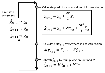
\includegraphics[width=10cm]{newmarkb.pdf}}
                \slantedcaption{Newmark-beta explicit time stepping scheme, as detailed for instance in \cite{Hug87}.}
                \label{fig:newmarkb}
            \end{figure}
%
            Figure \ref{fig:newmarkb} shows a diagram of a classical implementation of the Newmark explicit time scheme,
which is the implementation that is used in the SPECFEM software package that I will use in this thesis. At the beginning of each time step, the predictors are calculated from the
values of the potential at the previous time step. $M\ddot{\chi}_{n+1}$ is then obtained based on the sum of the stiffness term and of the force source term.
Finally, the value of $\hat{\dot{\chi}}_{n+1}$ is obtained
by multiplying the inverse of the mass matrix $M^{-1}$, which is pre-computed and stored at the initialization step of the entire simulation.
As in the SEM the mass matrix is perfectly diagonal, by construction of the SEM technique, that mass matrix is in fact a vector (i.e., only the diagonal of the mass matrix is non zero
and thus needs to be stored), and inverting it is straightforward, since the matrix is diagonal. Its inverse is thus also a simple vector.


\section{Supercomputers, High-Performance Computing (HPC), and the SPECFEM software package}

\subsection{Supercomputers and High-Performance Computing (HPC)}

Imaging what is inaccessible to direct observation, i.e. wave propagation and tomography / imaging in complex media, is a classical issue that encompasses many scientific and engineering domains, with a wide range of scientific as well as societal applications: non-destructive testing, acoustic probing, medical imaging, study of earthquake-prone regions and related seismic hazard, seismic imaging for oil and gas exploration, CO$_2$ storage and sequestration, geothermic energy... The key idea in these different imaging problems is to make use of the interactions of acoustic waves with the heterogeneities of the medium that they travel in to detect and characterize these heterogeneities. In order to address these different challenges, a necessary tool is high-performance computing (HPC) in order to be able to successfully achieve these calculations for real applications. Indeed, simulation has nowadays become the so-called third pillar of science, together with theory and experimentation, being critical for advancing our understanding of complex natural systems such as the oceans, the Earth, the atmosphere, and even the human body. Numerical modeling of acoustic wave propagation has a long history dating from the 1970s, but until a decade ago was reserved to computer experts with expensive dedicated equipment; it is now easily accessible to both academic and industrial laboratories. The success of the Partnership for Advanced Computing in Europe (PRACE) of the European Union has shown this very clearly, and the Horizon2020 program puts even more emphasis on that. Quoting the President of the European Union Jean-Claude Juncker, "mega data and high-performance computing favor economic growth as well as innovation and benefit all economic sectors as well as society as a whole, for science, research and sharing of knowledge". High-performance computing and big data are now converging, and the next big challenge we as a society are facing can be seen as High Performance Data Analytics (HPDA).

The first supercomputers appeared in the 1960s. What the word supercomputer stands for varies over time, because the most powerful computers in the world
at one point in time tend to be matched, and then surpassed, by other, more recent machines with sometimes different technology over the years.
The first supercomputers were simple single-processor computers.
In the 1970s, most supercomputers adopted a vector processor, which decoded an instruction once and applied it to a series of operands.
It was only towards the end of the 1980s that the technique of massively parallel systems was adopted, with the use of thousands of processors in the same supercomputer.

Currently, supercomputers are most often designed as unique models by traditional computer builders. Supercomputers are used for all tasks that require very high computing power, such as weather forecast, climate studies, modeling of chemical molecules, physical simulations (aerodynamic simulations, material resistance calculations,
simulation of nuclear weapon explosion, study of nuclear fusion, etc.), cryptanalysis, or simulations in finance and insurance.
Civil and military research institutions are among the largest users of supercomputers.
In France, these machines are found in national computational centers, such as the Grand \'Equipement National de Calcul Intensif (GENCI),
the Institut du d\'eveloppement et des ressources en informatique scientifique (IDRIS), the Centre informatique national de l'enseignement sup\'erieur (CINES),
the Tr\`es Grand Centre de Calcul (TGCC), the Commissariat \`a l'\'energie atomique et aux \'energies alternatives (CEA),
and also some large companies like Total, EDF or M\'et\'eo-France.

Nowadays, these computers are capable of processing and communicating very large volumes of data in a very short time.
Their design must ensure that this data can be read, transferred and stored quickly. If that were not the case, the computing power of the processors would be under-used (bottleneck).
The memory architecture of the supercomputers is thus studied and carefully optimized to continuously supply the data to each processor in order to make the most of its computing power.

Figure~\ref{fig:top500} shows that so-called petaflops supercomputers, i.e., parallel computers capable of calculating $10^{15}$ floating-point operations per second (see Table~\ref{table:petaflop_exaflop}), which are the current state-of-the-art technology\footnote{The speed of the current fastest supercomputer (as of February 2018) being about 93 petaflops, but supercomputers around 1 petaflops being more widely available.}, have become standard and easily available around 2018 (blue line), and that around 2020 the first exascale/exaflops machine (i.e., 1000 times faster than petaflops) will appear somewhere in the world (orange line). Even more importantly, it shows that it takes about nine years, from 2008 to 2017, for petaflop supercomputing to go from the largest machine in the world to something relatively easily available; thus the same will happen for exascale computing, which should therefore be easily available around 2029 or so. We are thus confident that the calculation techniques that we will develop in Chapter~4 of this thesis based on (currently) expensive 3D calculations on a large parallel computer will become standard in the future, because the machines to use them will become widely available.

    \begin{table}
        \centering
        \slantedcaption{The different standard names used for the speed of current and future supercomputers, illustrating their capacity (computational speed) in terms of the total number of floating-point operations they can compute in one second. Past names, in increasing order of speed, were: megaflop ($10^{6}$), gigaflop ($10^{9}$), teraflop ($10^{12}$).}
\vspace{5truemm}
        \begin{tabular}{lll}
        Name & Number of floating-point & Date of that technology \\
             & operations per second    &  \\ \hline
petaflop  & $10^{15}$ & current, since 2009 \\
exaflop   & $10^{18}$ & around 2020 \\
zettaflop & $10^{21}$ & around 2030? \\
yottaflop & $10^{24}$ & around 2040??
        \end{tabular}
        \label{table:petaflop_exaflop}
    \end{table}

\noindent
As mentioned by \cite{GrSt15} in their review article on the evolution of HPC, the future of high-performance computing is now being expressed and analyzed both from the point of view of how it will be implemented from a technological point of view and, more importantly, of the ways in which it will impact large fields in science and technology, commerce, industry, security and society. The trend of having increasingly more powerful supercomputers each year should continue, because in the past years, intra-node parallelism on high-performance computers has continuously been increasing, either because of the increasing number of processor cores available on CPUs, or because of accelerating computing units such as GPU graphics cards (GPU computing) or Intel accelerators (Intel Xeon Phi, Intel Many Integrated Core Architecture "Knights Landing" i.e. MIC KNL). This trend is particularly reflected in the latest TOP500 list that ranks the 500 fastest supercomputers in the world, in which the first two supercomputers are heterogeneous systems equipped with accelerators. In order to fully benefit from this hardware evolution, software packages and computing applications often require substantial modifications. Exascale machines will start to appear around 2020; with such machines, 3D calculations for wave propagation in complex nuclear reactor core models, as introduced in this thesis, will become something routinely used.

In this thesis, we will mostly use the French national OCCIGEN / GENCI (Grand \'Equipement National de Calcul Intensif) machine located at CINES (Centre Informatique National de l'Enseignement Sup\'erieur) in Montpellier, France. It is a parallel supercomputer built by the BULL Atos company that comprises 4212 Intel processors of the Haswell and Broadwell types with a total of 85824 processor cores, and a total of 283 terabytes of memory, with a peak processing speed of 3.5 petaflop per second. As of February 2018 it is the 54th largest supercomputer in the world.


    \subsection{The SPECFEM software package: A very efficient numerical code for acoustic or seismic wave propagation simulation}

SPECFEM is an open-source software package that can model acoustic or seismic wave propagation in complex media, using the spectral-element method.
The first versions of this codes were developed by Dimitri Komatitsch and Jean-Pierre Vilotte at Institut de Physique du Globe (IPGP) in Paris,
France from 1995 to 1997 and then by Dimitri Komatitsch and Jeroen Tromp at Harvard University and Caltech, USA for seismic wave propagation simulation.
It has more recently been applied to ultrasonic non-destructive testing and to ocean acoustics.
The code is being developed on Github (\url{http://github.com/geodynamics}), which is a development platform for open-source projects.
It is also available on the Computational Infrastructure for Geodynamics (CIG) platform, which is widely used in Earth Sciences.
2D, 2.5D (axisymmetric, \cite{Bottero2016Anaxisymmetrictime}) and 3D versions of the package are available.
The software package simulates acoustic or seismic wave propagation
at the local or regional scale and performs full waveform imaging (FWI) or adjoint tomography based upon the spectral-element method
(SEM).

            \begin{figure}[htbp]
                 \centerline{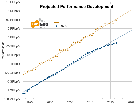
\includegraphics[width=13cm]{top500_list_evolution.pdf}}
                \slantedcaption{Speed of the fastest supercomputer in the world (in orange) and its projected evolution over the years, as well as the speed of the 500th, i.e. of a machine typical of moderate-size supercomputers easily available to researchers at regional or laboratory sites (in blue). The extrapolation is reliable, as shown by the very good fit over the first twenty years. In log scale, adapted from www.top500.org.}
                \label{fig:top500}
            \end{figure}

The SEM is a continuous Galerkin technique \citep{TrKoLi08,Peter2011Forwardandadjoint},
which can easily be made discontinuous \citep{BeMaPa94,KoWoHu02,ChCaVi03,LaWaBe05,Kop06};
it is then close to a particular case of the discontinuous Galerkin
technique \citep{ReHi73,LeRa74,HuHuRa99,RiWh03,DuKa06},
with optimized efficiency because of its tensorized basis functions
\citep{WiStBuGh10,AcKo11}. In particular, it can accurately handle very distorted mesh elements \citep{OlSe11}.
Effects due to lateral variations in compressional-wave speed, shear-wave
speed, density, and topography of object interfaces can all be included.
The package can accommodate full 21-parameter anisotropy
(see~\citet{ChTr07}) as well as lateral variations in attenuation
\citep{SaKoTr10}. Adjoint capabilities and finite-frequency kernel
simulations for imaging of unknown complex media are also included \citep{TrKoLi08,FiIgBuKe09,ViOp09,MoChKoWa15}.
In fluids, when gravity is turned off, SPECFEM3D uses the classical linearized Euler equation.
The goal in my thesis is to adapt and use this package to simulate ultrasonic wave propagation
in a sodium reactor core, for instance using approximations of such a complex propagation medium coming from thermal-hydraulic simulations
of such a core as performed by CEA using its TrioCFD software package (Figure~\ref{fig:specfem}).

        \begin{figure}[htbp]
                \centerline{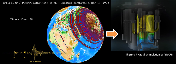
\includegraphics[width=17cm]{specfem.pdf}}
            \slantedcaption{The SPECFEM open-source software package that will be used in this thesis
was initially developed in seismology, to simulate the propagation of seismic waves propagating in the Earth following large earthquakes
(left, from the users manual of SPECFEM); the goal in this thesis is to adapt it and use it to simulate ultrasonic wave propagation
in a sodium reactor core, for instance using approximations of such a complex propagation medium coming from thermal-hydraulic simulations
of such a core as performed by CEA using its TrioCFD software package (right, from the CEA home page).}
            \label{fig:specfem}
        \end{figure}

It has very good accuracy and convergence properties \citep{Coh02,DeSe07,SeOl08,AiWa09,MeStTh12}.
The spectral element approach admits spectral rates of convergence
and allows exploiting $hp$-convergence schemes. It is also very well
suited to parallel implementation on very large supercomputers \citep{KoTsChTr03,TsKoChTr03,Peter2011Forwardandadjoint}
as well as on clusters of GPU accelerating graphics cards \citep{KoMiEr09,Komatitsch2010Highorderfinite,Kom11}.
Tensor products inside each element can be optimized to reach very
high efficiency \citep{DeFiMu02}, and mesh point and element numbering
can be optimized to reduce processor cache misses and improve cache
reuse \citep{KoLaMi08a}. The SEM can also handle triangular (in 2D)
or tetrahedral (in 3D) elements \citep{WinBoyd96,KoMaTrTaWi01,MeViSa06}
as well as mixed meshes, although with increased cost and reduced
accuracy in these elements, as in the discontinuous Galerkin method.

Figure \ref{fig:spec_flow} shows a typical workflow when simulating wave propagation in a complex model based on the SPECFEM software package.
The process is divided into four main steps: mesh creation, partitioning of the mesh created for parallel processing when running on a parallel computer,
simulation database generation, and final resolution and calculation of wave propagation (the so-called solver step).
For explicit time marching, the user can freely choose between different schemes:
second-order Newmark scheme \parencite{Newmark1959Amethodof}, fourth-order four-stage classical
Runge-Kutta \parencite{Butcher2016Numericalmethodsfor}, or fourth-order six-stage LDDRK (Low-Dissipation and low-Dispersion Runge-Kutta)
\parencite{Berland2006Lowdissipationand}. Available mesh types (in terms of geometry of the mesh elements) are 4-node and 9-node quadrangular elements
in the 2D case and 8-node and 27-node hexahedral elements in the 3D case.
For mesh creation, a simple (relatively basic) internal mesh creation tool is provided, but any external mesh creation tool that can produce hexahedral meshes can also
be used, for instance CUBIT/Trelis (developed by Sandia National Laboratories, USA) or Gmsh \parencite{Geuzaine2009Gmsh:A3}.
In the case of infinite or semi-infinite media, the code implements Convolution or
Auxiliary Differential Equation Perfectly Matched absorbing Layers
(C-PML or ADE-PML) \citep{KoMa07,Komatitsch2008Anunsplitconvolutional,MaKoGeBr10}.

\clearpage

        \begin{figure}[htbp]
            \centerline{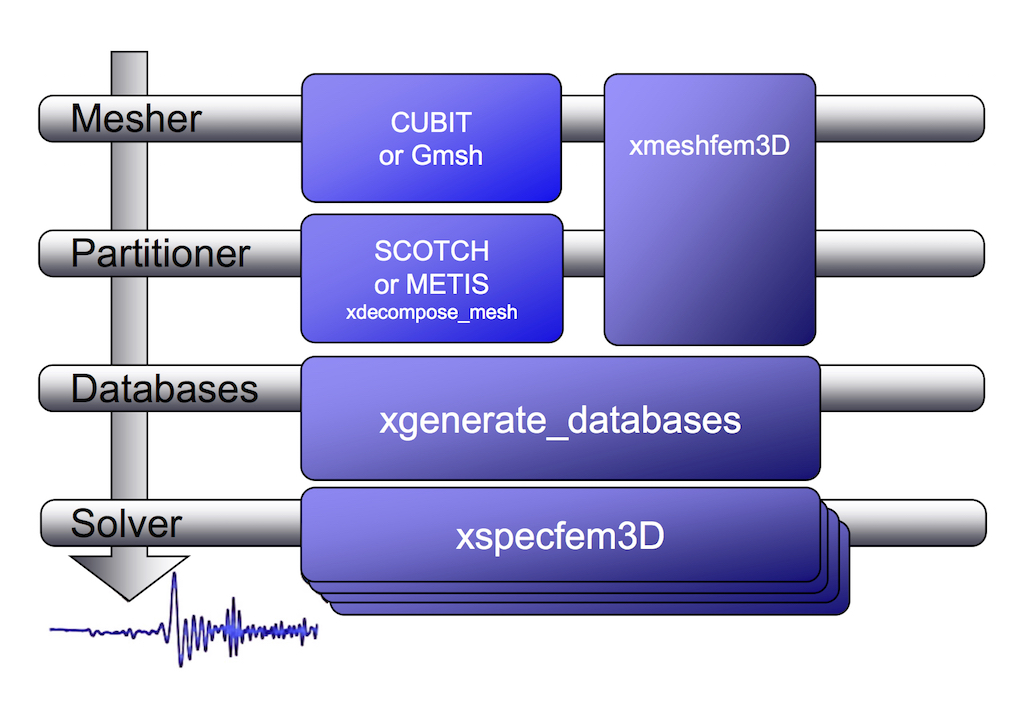
\includegraphics[width=12cm]{spec_flow.jpg}}
        \slantedcaption{Workflow of a typical wave propagation calculation when using the SPECFEM software package.
The process is divided into four main steps: mesh creation, partitioning of the mesh created for parallel processing when running on a parallel computer,
simulation database generation, and final resolution and calculation of wave propagation (the so-called solver step). Taken from the users manual of SPECFEM.}
        \label{fig:spec_flow}
        \end{figure}

The SEM was originally developed in computational fluid dynamics \citep{Patera1984Aspectralelement,MaPa89}
and has been successfully adapted to address problems in seismic wave
propagation. Early seismic wave propagation applications of the SEM,
utilizing Legendre basis functions and a perfectly diagonal mass matrix,
include \citet{CoJoTo93}, \citet{Kom97}, \citet{FaMaPaQu97},
\citet{KoVi98} and \citet{KoTr99}, whereas applications involving
Chebyshev basis functions and a non-diagonal mass matrix include \citet{SePr94}, \citet{PrCaSe94} and \citet{SePrPr95}.
In the Legendre version that we use in SPECFEM the mass matrix is purposely slightly inexact but diagonal (but can be made exact if needed, see \cite{Teu15}),
while in the Chebyshev version it is exact but non diagonal.
For a detailed introduction to the SEM as applied to regional seismic
wave propagation, one can refer to \citet{KoVi98,KoTr99,ChKoViCaVaFe07,TrKoLi08}
and even more specifically to \citet{Lee2009Effectsoftopography,LeChKoHuTr09}.
A detailed theoretical analysis of the dispersion
and stability properties of the SEM is available in \citet{Coh02}, \citet{DeSe07}, \citet{SeOl07} and \citet{MeStTh12}.

In a spectral-element method, some spurious modes, which have some similarities with classical so-called "Hourglass modes" in finite-element techniques,
although in the SEM they are not zero-energy modes, can appear in some (but not all) cases in the spectral element in which the source is located.
Fortunately, they do not propagate away from the source element.
However, this means that if you put a receiver in the same spectral element as a source, the recorded signals may in some cases be wrong, typically exhibiting some spurious
oscillations, which are often even non causal.
If that is the case, an easy option is to slightly change the mesh in the source region in order to get rid of these Hourglass-like spurious modes,
as explained in \cite{DuLiScGa14}, in which this phenomenon is described in details, and in which practical solutions to avoid it are suggested.

\clearpage

All SPECFEM software is written in Fortran2003 with full portability
in mind, and conforms strictly to the Fortran2003 standard. It uses
no obsolete or obsolescent features of Fortran. The package implements parallel
programming based upon the Message Passing Interface (MPI) \citep{GrLuSk94,Pac97}.

The code is particularly well suited to very large parallel supercomputers.
SPECFEM3D won the prestigious Gordon Bell international computer science award for best performance at the SuperComputing~2003
conference in Phoenix, Arizona (USA) \citep{KoTsChTr03}.
It was a finalist again in 2008 for a run at 0.16 petaflops (sustained) on 149,784 processors
of the `Jaguar' Cray XT5 system at Oak Ridge National Laboratories
(USA) \citep{CaKoLaTiMiLeSnTr08}. It also won the BULL Joseph Fourier supercomputing award in 2010.
It reached the sustained one petaflop performance level for the first time in February 2013
on the Blue Waters Cray supercomputer at the National Center for Supercomputing Applications (NCSA), located at the University of Illinois at Urbana-Champaign (USA).

